\begin{figure}[t]
\centering
\begin{subfigure}[t]{0.49\linewidth}\centering
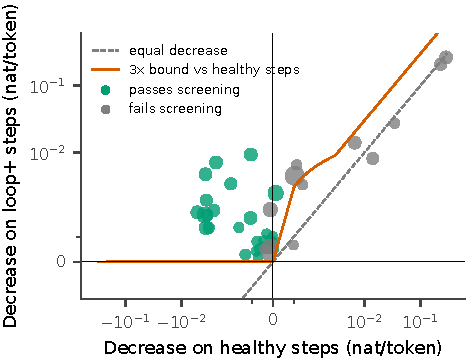
\includegraphics[width=\linewidth]{figs/offline_selectivity.pdf}
\caption{Offline screening of \mwOffNCand{} weight edits.}
\end{subfigure}\hfill
\begin{subfigure}[t]{0.49\linewidth}\centering
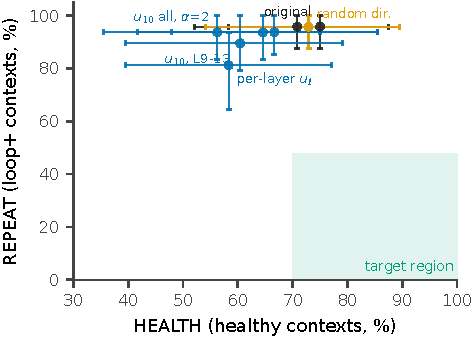
\includegraphics[width=\linewidth]{figs/steering_pareto.pdf}
\caption{Behavioural steering arms.}
\end{subfigure}
\caption{\textbf{On the 0.8B, edits large enough to matter hit healthy actions as hard as loops.} (a)~Teacher-forced decrease in log-probability of the recorded action, loop versus healthy steps, on 40 fixed development contexts (symlog axes; marker area grows with the number of weights edited). % source: data/pod_astra/REPORT.md rounds 1-2 (40 fixed contexts)
The red line is the screening bound against healthy steps (loop decrease at least 3 times the healthy decrease); the criterion applies the same bound to loop$-$ and successful steps, so \mwOffGreyAbove{} failing candidates lie above the line. Every passing candidate lies above it, with loop decreases of at most \mwOffQualMaxLoop{} nat/token. (b)~Loop rate versus healthy-action rate per steering arm, 95\% bootstrap CIs over contexts \citep{efron1979bootstrap}. The shaded region is the pre-registered target, and no arm enters it.}
\label{fig:mw}
\end{figure}
